\section{绪论}

\subsection{选题背景}
互联网技术的蓬勃发展在很大程度上给人们的生活带来了越来越多的便利,人们在逐渐适应网络这样的平台的同时,也更倾向于甚至依赖在网络平台上完成生活中的各种事情,可以说,网络对于人们的重要性已经几乎等同于空气、水和食物。按照网络平台的功能来划分,门户网站(新浪、搜狐等)是新闻实事评论发布的主要渠道,社交网站(微博、人人等)是人们分享个人想法和心情的首选,博客系统(新浪博客、百度空间等)是人们发表和传达思想和经验的主要平台,以及一些新新涌现的图片和视频等多媒体资源分享平台(优酷土豆、POCO等)大大丰富了人们的娱乐生活。此外,鉴于国内发达的物流行业,各大电子商务平台(淘宝、京东等)也使得不用出门就能购物成为了现实。按照网络平台资源的载体来划分,包括文本、图片、音乐和视频几大类,其中文本无疑是整个互联网资源的主体,无论是传统的新闻、博客、评论、说明,还是新新发展的弹幕视频网站(Acfun\footnote{http://www.acfun.tv/}、Bilibili\footnote{http://www.bilibili.com/}等),都是由很多文本信息组成的。按照网络平台的用户参与角度来划分,可以将用户角色分为两种:信息发布者和信息获取者。以程序员为例,当他需要学习一项新技术时,往往会通过搜索引擎寻找一些与该技术相关的教学经验文章,从而使自己尽快掌握该项技术。等对该技术数量掌握之后,往往又会通过写技术博客的方式记录下他的学习历程和使用中的经验之谈,以供他人参考。同时,该用户还肯定拥有其他多个兴趣爱好,比如他可以与网上其他用户分享旅游游记、摄影作品等等。

虽然这些网站系统在功能上、信息载体上或是用户参与方式上都截然不同,但是宏观来看他们都存在一个共同的问题:信息孤岛现象。如图\ref{fig:problem}所示,当这些网站发展越来越多之时,各个网站之间信息不流通的问题也日渐明显,每个网站独立发展,出于安全性等方面的考虑,其资源和用户的数据并不能实现跨平台共享,从而使得每个网站成为一座座信息孤岛。

\begin{figure}[ht]
\centering
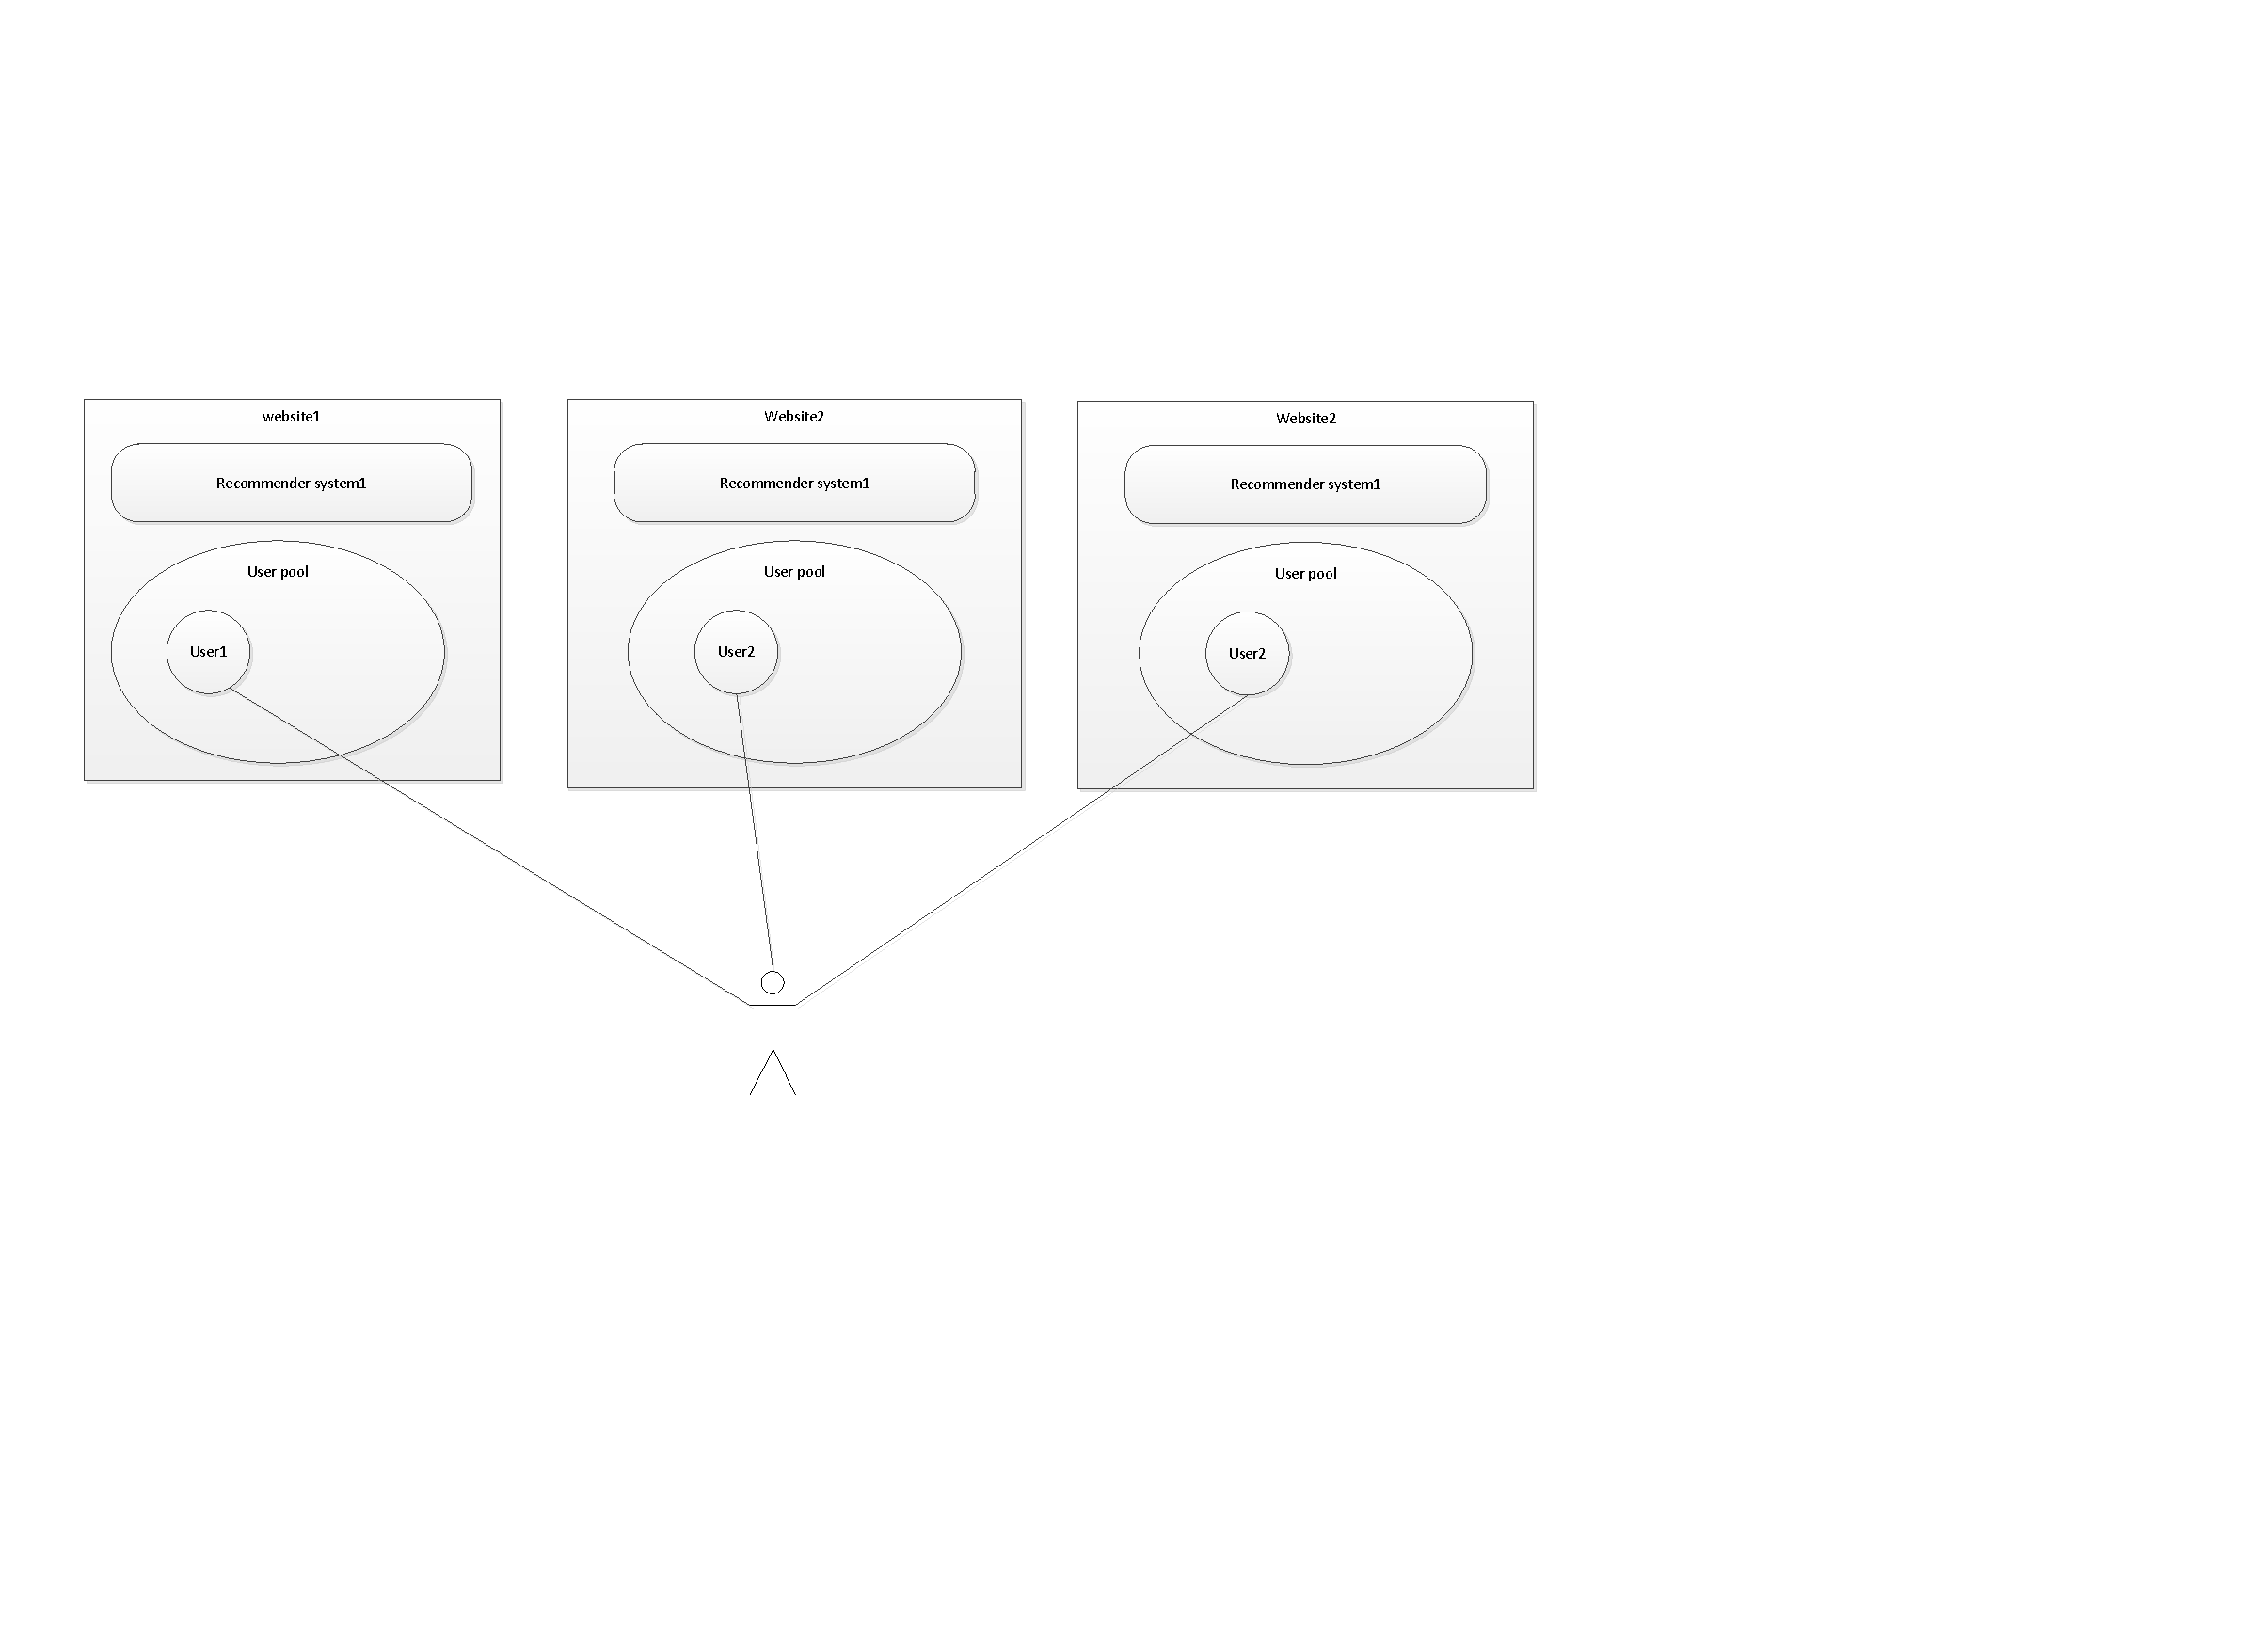
\includegraphics[width=\textwidth]{problem.pdf}
\caption{互联网平台的信息孤岛现象}
\label{fig:problem}
\end{figure}

举例来说,当用户作为信息获取者时,虽然每个网站可以为本平台上的用户提供很好的用户体验,通过数据挖掘等技术发现用户的兴趣,为其推荐有潜在需求的信息,但是不同网站之间的用户兴趣不能共享,导致兴趣推荐的不准确。当用户作为信息发布者时,其操作会更加繁琐,他往往需要打开多个网站重复几乎相同的操作来发布同样的内容,最明显的证据就是同时使用微信、微博和人人的用户需要在三个平台上重复三次操作完成发布。当这些网站越来越多的时候,问题也随之而来,即用户可能需要打开很多个独立的网站来完成一系列类似的事情。比如,先在新闻网站上浏览最新发生的时事,接着在摄影网站上发布新照片,然后在社交网站上浏览好友更新的状态,最后在电商网站上购买一些商品等等。换句话说,用户是单向地去寻找想要的信息,这其中无疑包含了一些不必要的重复操作。退一步来说,即使存在某些用户只在社交网站上浏览信息,很少接触其它网站,也会有一些重复操作的问题。因为该用户的好友很有可能是分散地活跃于各个不同的社交网站平台(微博、人人网等),而且每个平台发布的信息肯定有所不同,所以该用户仍然需要逐个登录各个网站后才能浏览到各个用户的信息。再退一步说,即便现在已经有些软件把所有社交网站整合成一个统一接口,让用户只需一次登录就能同时访问多个平台,用户仍然会遇到信息冗余的问题,比如重复的新闻、不感兴趣的推荐等等。

为了解决上述问题,我们设想有这样一个智能系统:每当用户打开系统时,系统会自动推送今天的时事新闻、其好友最近更新的状态、感兴趣或者正在促销的商品,以及一些根据用户偏好过滤的信息。此外,他也可以在系统上发布自己的信息给他的好友,甚至给那些对他信息感兴趣的陌生人。虽然,实现这样一个系统的工作量和难度是巨大的,但仔细观察后可以发现这样一个重要的规律:即用户希望所有的信息能够在整个互联网上智能地自主流动,在用户单方面寻找信息的同时,让信息也能自主地流向符合特定需求的用户。

\begin{figure}[ht]
\centering
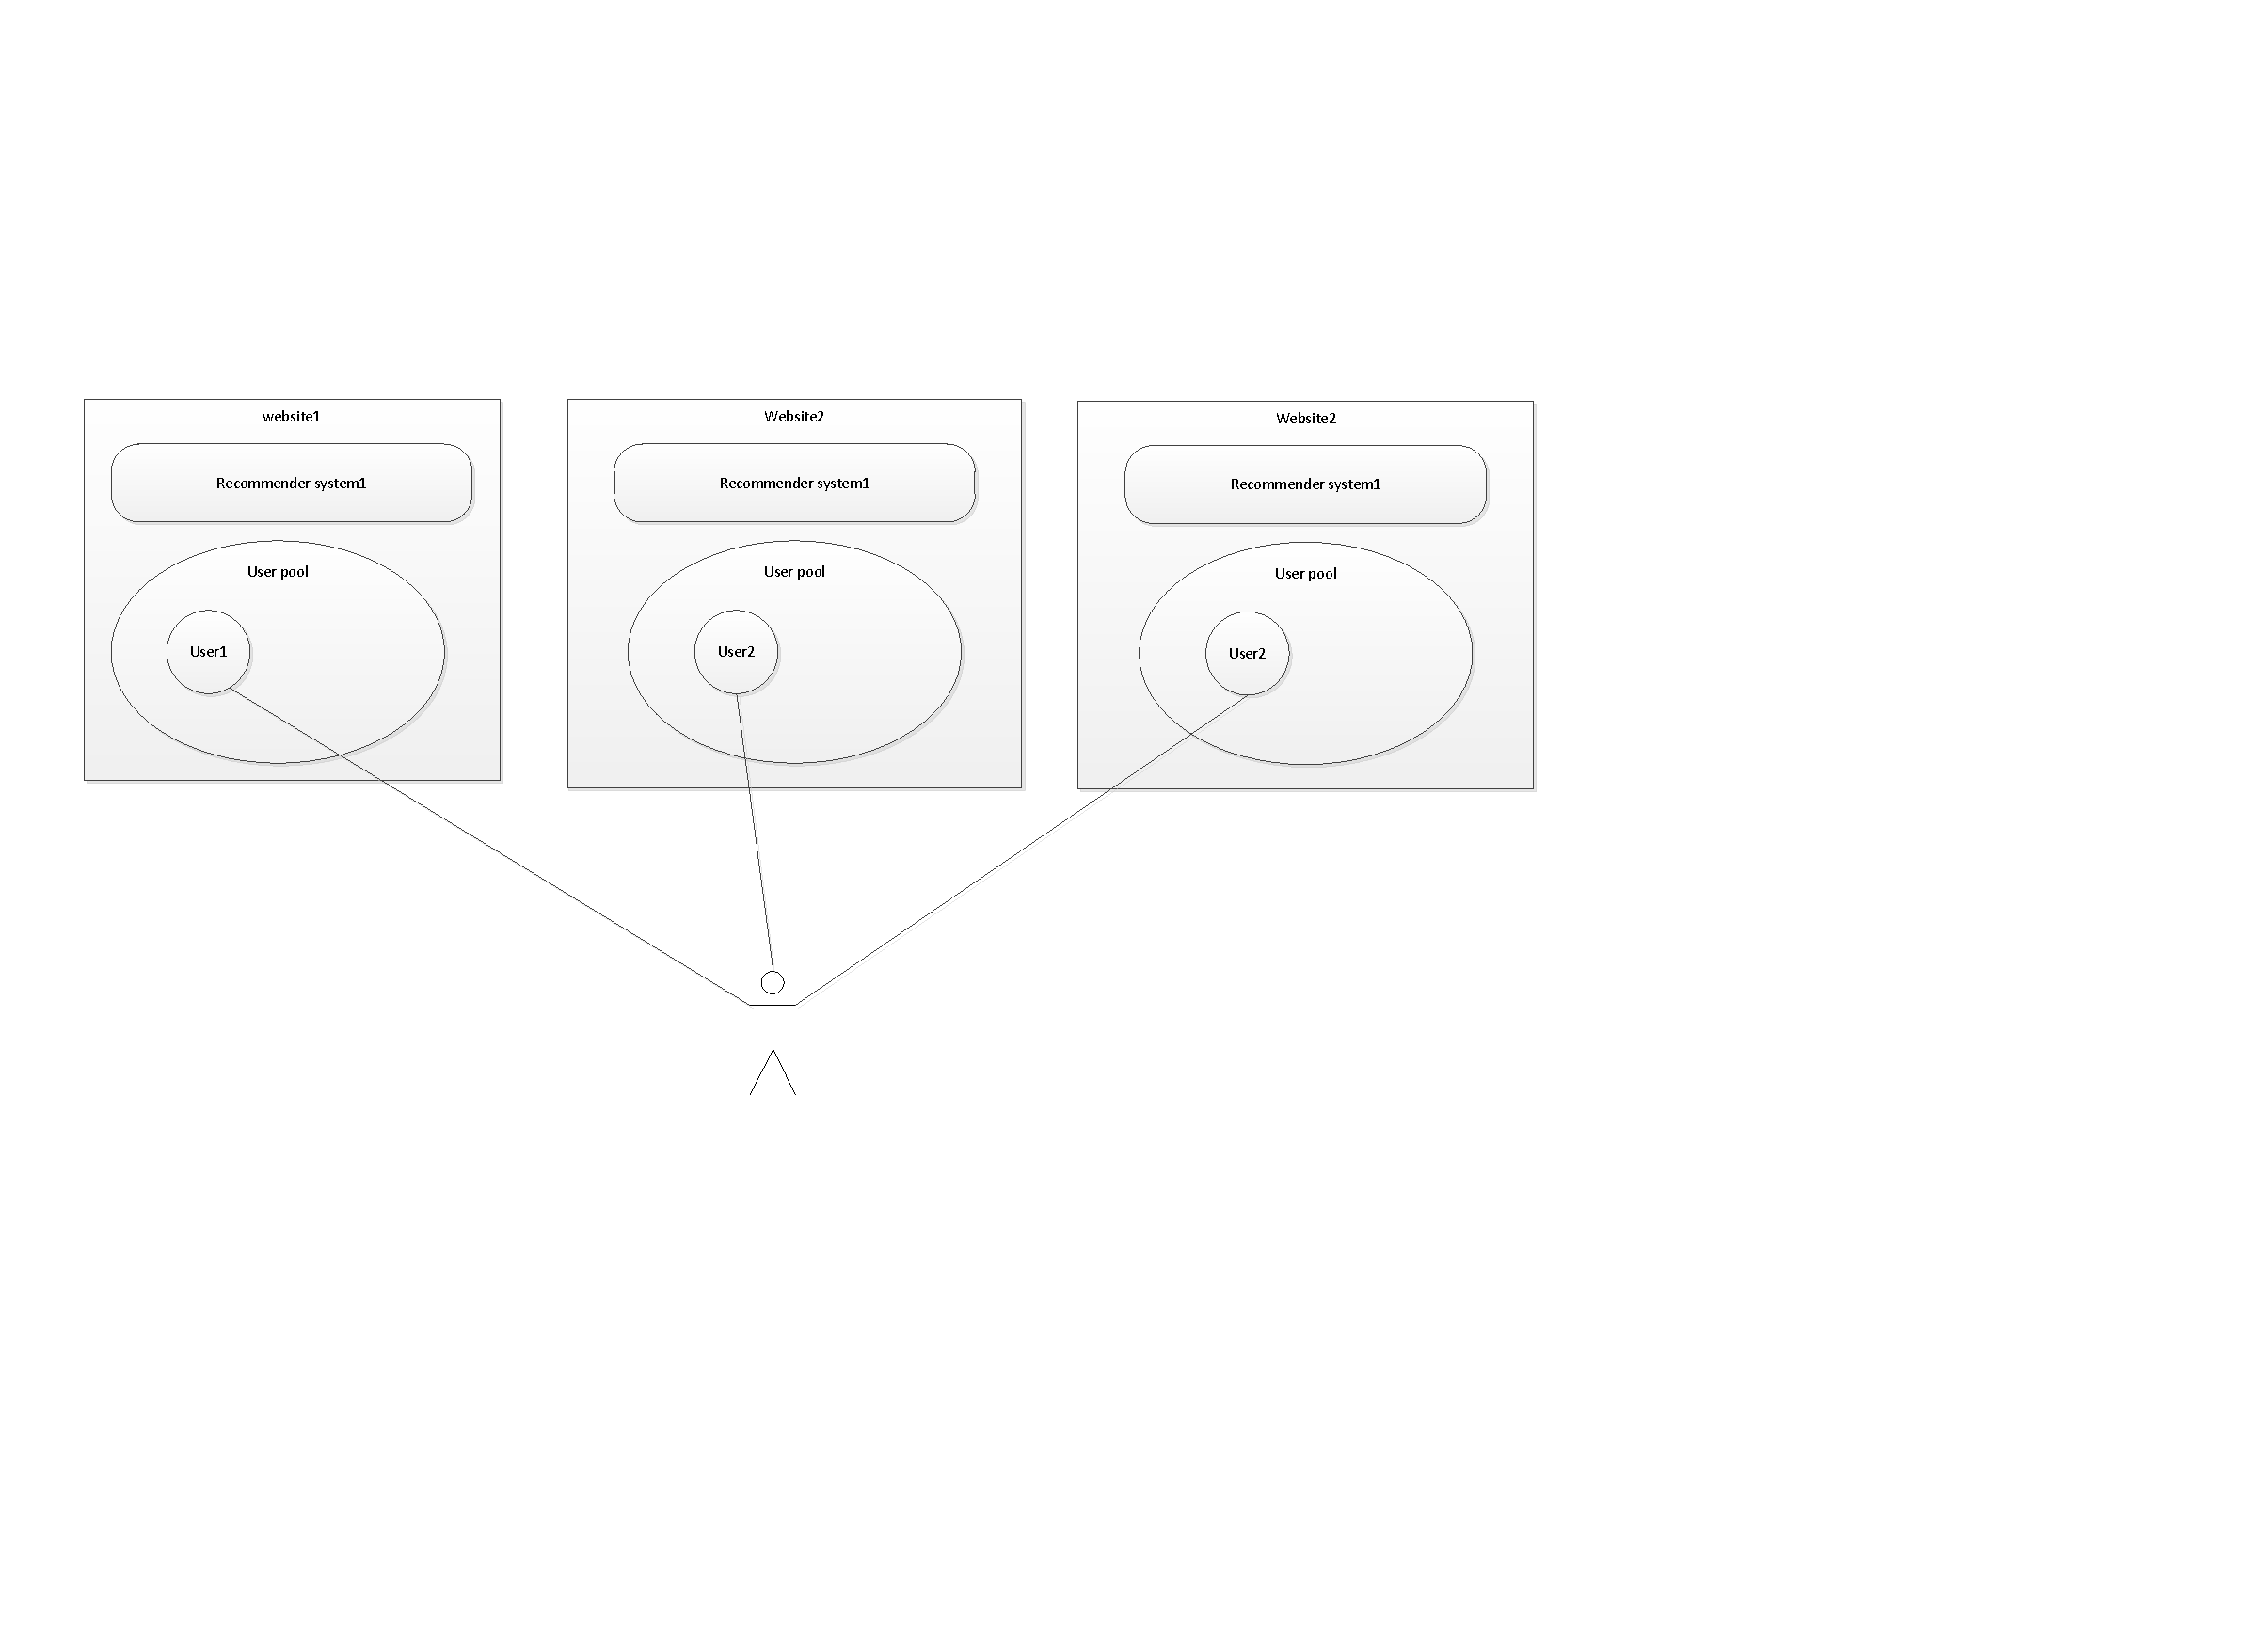
\includegraphics[width=\textwidth]{problem.pdf}
\caption{一种基于P2P网络的智能系统解决方案}
\label{fig:solution}
\end{figure}

从抽象层面来看,要实现这样一套信息自主流动的机制,传统的集中式计算模式已经不再适用。如图\ref{fig:solution}所示,这里每个用户均看作一个独立的节点,所有的节点整合在一起就形成一个巨大的P2P网络。其中,每个节点既充当服务器用于分发信息,也充当客户端用于接收信息,并且由某个节点发出的信息在其它节点间传播的时候会自主流动,寻找潜在的、匹配的节点。简单来说,要使信息能够自主流动,就要攻克这几方面的难点:

\begin{itemize}
\item 资源信息描述与匹配:互联网资源普遍呈现出半结构化或非结构化的特征,以普通的新闻或者博客为例,除了作者、标题、时间等结构化信息,正文纯文本都是典型的非结构数据。因此, 如何从这些非结构化的文本信息中提取出有用的特征、并用这些特征来衡量这些文本之间的相关性是本文重要研究内容。
\item 用户兴趣挖掘与关联:用户的兴趣可以从其发布和查看的信息中反映出来,基于上述对资源信息的描述模型,可以训练出某一时刻或者某一时段内的用户兴趣。但是,由于用户兴趣可能会随着时间的推移而不断变化,并且在同一时刻可能同时存在长期兴趣和短期兴趣。因此,这部分需要基于资源模型来解决用户兴趣随时间变化的问题。
\item P2P网络路由与搜索:从整个网络结构来看,在初始状态下各个用户节点之间的关系仅仅为物理意义上的距离关系,换句话说,节点与节点之间的边的权重不能代表用户与用户之间兴趣的相似度,从而也就导致每个节点上的信息不能自由传播。因此,这部分需要借助用户兴趣模型,通过P2P网络的路由搜索算法来寻找潜在的相似节点,最后构成某一时间段内的稳定结构。 
\end{itemize}

\subsection{研究意义与应用价值}
对于上述提出的信息孤岛现象是主要由目前网站之间相互独立而导致的,这些中心化结构的独立网站架构存在以下几个问题:

\begin{itemize}
\item 从资源传播的角度来看,每个网站的数据都仅仅在一个局部范围内可用,但是用户却要在多个这样的局部范围内同时使用多个网站。虽然对于每个网站可以维护相对较好的资源整合和管理,但是对于属于用户的资源的传播带来了很大的阻碍。
\item 从计算资源的角度来看,每个独立的传统B/S架构的网站通常由背后的一套计算群组来支撑,当网络流量十分巨大的时候,服务器的硬件和软件性能决定了系统平台可承受的最大程度。而在用户这边的客户端的I/O消耗相对小很多,但是大量客户端的请求对于服务器是一个不小的考验,从而导致了服务器成为整个系统的计算瓶颈。
\item 从隐私安全的角度来看,目前网站的数据均由平台自己的数据库进行维护,对于数据泄露成为重大隐患之一,即使网站的安全性是非出色,用户也会担心其数据是否会被第三方利用于商业用途。
\item 从拓扑架构的角度来看,用户与网站系统组成了中心化的拓扑结构,该结构不利之处在于当网站服务器宕机或者网络中断的时候,所有用户均无法访问该系统,这就使得网站系统的备份机制与主从切换机制十分完善,而对于大部分初创公司的流量有限和资金不足等特征是一个很大的考验。
\end{itemize}
  
与中心化结构网站架构不同,在基于P2P网络架构中,每个节点都可以既可以充当服务器为其它节点提供资源,也可以作为客户端向其它节点获取资源。综合来说,P2P网络的应用具有以下几大优点\cite{p2psurvey}:

{\color{red} 以下需要同义重写}
\begin{itemize}
\item 非中心化:网络中的资源和服务分散在所有结点上,信息的传输和服务的实现都直接在结点之间进行,可以无需中间环节和服务器的介入,避免了可能的瓶颈。P2P的非中心化基本特点,带来了其在可扩展性、健壮性等方面的优势。
\item 可扩展性:在P2P网络中,随着用户的加入,不仅服务的需求增加了,系统整体的资源和服务能力也在同步地扩充,始终能比较容易地满足用户的需要。理论上其可扩展性几乎可以认为是无限的。例如:在传统的通过FTP的文件下载方式中,当下载用户增加之后,下载速度会变得越来越慢,然而P2P网络正好相反,加入的用户越多,P2P网络中提供的资源就越多,下载的速度反而越快。
\item 健壮性:P2P架构天生具有耐攻击、高容错的优点。由于服务是分散在各个结点之间进行的,部分结点或网络遭到破坏对其它部分的影响很小。P2P网络一般在部分结点失效时能够自动调整整体拓扑,保持其它结点的连通性。P2P网络通常都是以自组织的方式建立起来的,并允许结点自由地加入和离开。
\item 高性价比:性能优势是P2P被广泛关注的一个重要原因。随着硬件技术的发展,个人计算机的计算和存储能力以及网络带宽等性能依照摩尔定理高速增长。采用P2P架构可以有效地利用互联网中散布的大量普通结点,将计算任务或存储资料分布到所有结点上。利用其中闲置的计算能力或存储空间,达到高性能计算和海量存储的目的。目前,P2P在这方面的应用多在学术研究方面,一旦技术成熟,能够在工业领域推广,则可以为许多企业节省购买大型服务器的成本。
\item 隐私保护:在P2P网络中,由于信息的传输分散在各节点之间进行而无需经过某个集中环节,用户的隐私信息被窃听和泄漏的可能性大大缩小。此外,目前解决Internet隐私问题主要采用中继转发的技术方法,从而将通信的参与者隐藏在众多的网络实体之中。在传统的一些匿名通信系统中,实现这一机制依赖于某些中继服务器节点。而在P2P中,所有参与者都可以提供中继转发的功能,因而大大提高了匿名通讯的灵活性和可靠性,能够为用户提供更好的隐私保护。
\item 负载均衡:P2P网络环境下由于每个节点既是服务器又是客户机,减少了对传统C/S结构服务器计算能力、存储能力的要求,同时因为资源分布在多个节点,更好的实现了整个网络的负载均衡。
\end{itemize}
{\color{red} 重写结束}

基于上述有点,本文首先建立一套用于描述互联网信息和用户行为偏好的模型,旨在将这些具体的信息和用户行为偏好上升到抽象层面,剥离出一个统一的输入输出接口。对于那些专注于复杂的数据分析和建模工作的模块,该接口起到了整合的作用。而且,在此之后,也可以展开专门基于该描述模型的信息与用户匹配算法的研究。其次,根据上述信息描述模型与用户行为偏好模型的特点,从拓扑结构,通信机制等方面入手,建立一套合适的分布式架构(如P2P的计算模式),并利用上述的匹配算法,研究由各个节点组成的覆盖网络间的信息自主流动的机制。最后,将上述两项内容结合在一起,实现一套完整的信息自主流动的原型系统。

\subsection{国内外研究现状}
从目前的科学研究和商业应用方面来看,还没有关于一套基于P2P网络的信息自主流动机制的相关工作。因此,这部分将从文本信息挖掘、用户兴趣关联以及P2P网络搜索等三方面来具体展开阐明已有的研究工作。

在文本信息挖掘方面,由于当今的硬件和软件技术在各方面都有大幅度提高,产生了大量的不同类型的数据资源\cite{8},特别是纯文本的数据。这些文本大多来自于社交网络、新闻博客等网站,内容形式对于人们来说也是十分的丰富。但是这对机器来说却没有那么容易识别,因此需要设计一系列的算法来从这些文本数据中找出一些模式和规律,从而让机器更好地利用这些数据为人们创造更大的价值。结构化数据(Structured Data)通常可以存储在各类数据库中,但是纯文本数据却因为它的非结构化从而只能有通过搜索引擎等技术才能进行索引和查找\cite{5}。搜索引擎是信息检索(Information Retrieval)中的一种方式,其作用是方便用户直接通过输入关键词找到内容相关的文档集合,其目标是如何通过有效和高效的方法是检索的结果更加精确,涉及的研究领域包括文本聚类、文本分类、文本概括、推荐系统等\cite{12,9,7}。但是,在本文中,除了这些信息检索基本的需求,更重要的是从文本中挖掘出重要的特征和模式,将原本非结构化的数据量化成半结构化数据,并且这种量化过程更多地从用户兴趣这点切入的。针对这个要点,文本挖掘技术一般可以分为以下几大类:

\begin{itemize}
\item 文本提取(Text Extraction):
\item 文本概括(Text Summarization):
\item 文本降维(Dimensionality Reduction):
\item 文本的非监督学习方法(Unsupervised Learning):
\item 文本的有监督学习方法(Supervised Learning):
\item 文本的概率方法(Probablistic Method):
\end{itemize}

\subsection{本文内容安排}
本文的主要内容安排如下。首先本章对该研究的背景,主要研究内容和研究意义与研究现状进行了一个总体的介绍。第二章将对基于P2P网络的信息自主流动机制提出一个完整的技术方案,并且结合研究现状和存在的问题对设计需求和挑战进行详细描述,从而给出关键的技术点。第三章将对解决方案中的第一部分即文本资源的描述与匹配问题进行深入分析,通过结合现有成熟的模型,提出一整套全面的理论模型。第四章将结合第三章的研究基础对用户兴趣进行建模,结合现实中兴趣的动态变化特征给出相应的解决方案。第五章将基于第四章的研究基础提出一种基于P2P网络的路由与搜索算法,从而实现动态构建兴趣覆盖网络。第六章将根据第三、四、五章的理论进行模拟实验和真实实验,验证上面提出的新的方法的有效性。第七章则基于前文的研究成果实现了一套简单的智能系统原型,包括功能设计和系统架构等方面。最后第八章对本研究做了一个总结,并对研究进一步的工作方向进行了讨论。

